\documentclass[5p,sort&compress]{elsarticle}	

% THIS IS THE SETUP FROM NIRIS TEMPLATE

\newcommand{\RomanNumeralCaps}[1]
{\MakeUppercase{\romannumeral #1}}
\makeatletter
\def\ps@pprintTitle{%
  \let\@oddhead\@empty
  \let\@evenhead\@empty
  \def\@oddfoot{\footnotesize\itshape
    \hfill\today}%
  \let\@evenfoot\@oddfoot}
\makeatother
\usepackage{dcolumn}
\usepackage[utf8]{inputenc}
\usepackage[T1]{fontenc}

\usepackage{textcomp}
\usepackage{lmodern}
\renewenvironment{abstract}{\global\setbox\absbox=\vbox\bgroup
  \hsize=\textwidth\def\baselinestretch{1}%
  \noindent\unskip\textbf{Abstract}
  \par\medskip\noindent\unskip\ignorespaces}
{\egroup}
\usepackage{amsmath}
\usepackage{amssymb}
\usepackage{caption} %% figurer fugler
\usepackage{bm}
\usepackage{siunitx}
\sisetup{
  exponent-product = \cdot,
  output-decimal-marker  =  {.}, % komma-stil
  separate-uncertainty = false, %true hvis du ikke vil ha usikkerhet i parentes
  per-mode = symbol,
  group-digits = false,
}
\usepackage{graphicx}
\renewcommand{\topfraction}{.85}
\renewcommand{\bottomfraction}{.7}
\renewcommand{\textfraction}{.15}
\renewcommand{\floatpagefraction}{.66}
\setcounter{topnumber}{3}
\setcounter{bottomnumber}{2}
\setcounter{totalnumber}{10}
\usepackage{flafter}
\usepackage{booktabs}
\usepackage{multirow}
\usepackage{hyperref}
\usepackage{cleveref}
\usepackage{comment}
\usepackage{arydshln}
\usepackage[font=small,labelfont=bf]{caption}
\usepackage{subcaption}

% Dakrmode
\usepackage{xcolor}
% \pagecolor[rgb]{0.128, 0.128, 0.128}  %black
% \color[rgb]{0.848, 0.848, 0.848}  %grey

% \urlstyle{same} % makes the url look like the text, still clickable and colored
\hypersetup{
  colorlinks=true,
  linkcolor=purple,
  filecolor=magenta,
  urlcolor=cyan,
  citecolor=purple
}



\begin{document}
\begin{frontmatter}

  \title{TFE4575: Fabrication of 675 nm wavelength LEDs}
  %\title{bonustitle}

  \author[fysikk]{Brynjar Morka Mæhlum}
  \author[fysikk]{Thord Niri Gjesdahl Heggren}
  \address[fysikk]{Department of Physics, Norwegian University of Science and Technology, 7491 Trondheim, Norway.}

  \begin{abstract}

    \noindent Light emitting diodes (LED) are widely used light producing electrical components.
    Producing LEDs is a micro- and nanotechnological processes.
    In this report, a premade multi-layered semiconductor wafer is used to produce LEDs.
    The wafer have been processed by strategically using photolithography, deposition, and etching.
    The LED have been characterized using an optical microscope, a scanning electron microscope, a profilometer, an ellipsometer and a SourceMeter.
    The characterizations revealed that some process steps resulted in minor defects.
    However, measurements of the IV-characteristics of the LEDs have been performed, and it confirmed that the LEDs are working as diodes.
    With voltage at 1.7 V and current at 30 mA the LEDs emits red light, which is the around the target wavelength of 675 nm.
    % Producing the LEDs did not always go as planned, and some defects and artifacts were produced.

  \end{abstract}


\end{frontmatter}

{ % This changes links to purple instead of blue
\hypersetup{linkcolor=purple}

\tableofcontents

%%% dette gjenstår:
% conclusion
% fikse layout 

% abstract
% IV i diskusjon
% IV measurements
% IV i metode
% IV i resultater


%%%%%%%%%%%%%%%%%%% INTRODUCTION %%%%%%%%%%%%%%%%%%
\section{Introduction}
\label{intro}
% INTRODUCTION

LEDs (Light Emitting Diode) are, as the name suggests, a type of electrical component producing light. 
They are widely used due to their low power consumption, long lifetime, small size, and fast switching \cite{unknown}.
LEDs are made up of strategically layered semiconductors and metals.
Then, in order to produce a working diode, the wafer needs to undergo several process steps.
Some of these can be photolithography, etching, deposition, and annealing.
After, the LEDs should be characterized and tested, e.g. by scanning electron microscopy (SEM), optical microscopy and current-voltage (IV) testing.



% LEDs are important nanotechnology products, which is why making a LED was the lab task in TFE4575.
% While doing this lab the students used many nanotechnology techniques to produce a LED from a metal stack.
% Lithography, etching, deposition, characterization, and more were used to produce a LED.
% These techniques should be familiar for the nanotechnology students specializing in nanoelectronics at NTNU, and is why they were chosen for this lab.
% As stated in the introduction lecture, doing photolithography requires training with failing to be able to do it correctly.
% In almost every single lab session, the students managed to fuck up a big or a small step, resulting in a lot of learning and redoing.
% However, the students managed to produce a working LED in the end, and the lab was a great success.
% The LED will be sold to the highest bidder, or be used as the star in Thords Christmas tree.
% Merry Christmas, we hope you enjoy the read!'


%%%%%%%%%%%%%%%%%%% THEORY %%%%%%%%%%%%%%%%%%
\section{Theory}
\label{theory}
% THEORY

\subsection{LED theory}
\label{LEDtheory}
LEDs are made of a PN junction, which is a semiconductor junction between a p-type and an n-type semiconductor.
The p-type semiconductor is doped with a lot of holes, and the n-type semiconductor is doped with a lot of electrons.
The junction is made by doping the semiconductor with impurities, which are atoms that are not part of the semiconductor crystal.
The impurities are added to the semiconductor to change the electrical properties of the semiconductor.
Light is emitted when an electron jumps from the n-type semiconductor to the p-type semiconductor.
More on semiconductor physics can be found in \cite{streetman2015solid}.


\subsection{Photolithography}
\label{photolithography}

Photolithography is used to make micro- and nanoscale structures on a substrate.
The process is done in a cleanroom, where the air is filtered to remove dust and other particles.
Small contamination can ruin the process by disturbing the resist.
The photoresist is a polymer that is sensitive to light, which will either harden or dissolve depending on the type of photoresist.
This is the steps of the process, and the reason for each step:

% cleaning, spinn coating, soft bake, exposure,  develop, post exposure, hard bake, inpect

\begin{enumerate}
    \item \textbf{Cleaning}: Remove any contamination from the substrate.
    \item \textbf{Spin coating}: Spin coat the photoresist on the substrate.
    \item \textbf{Soft bake}: Bake the photoresist to remove any solvent.
    \item \textbf{Exposure}: Expose certain areas of the photoresist to light. Eventually with mask alignment.
    \item \textbf{Develop}: Develop the photoresist to remove the softened parts.
    \item \textbf{Post exposure bake}: Bake the photoresist to enhance adhesion. \textcolor{red}{??}
    \item \textbf{Hard bake}: Bake the photoresist to remove any solvent. Not often needed.
    \item \textbf{Inspect}: Optical inspect the photoresist to see if it is good.
\end{enumerate}

Negative photoresist are often used for lift-off, because negative photoresist can achieve an undercut which can improve the metallization edges.
Photoresists needs different developing time and exposure doses, and they do change over time when the photoresist is exposed to light, heat, humidity, and time.



\subsection{Etching?}
\label{etching}


\subsection{Characterization equipment}
\label{characterization}

The characterization equipment used in this lab was optical microscope, SEM, profilometer and IES-stuff to measure the LED efficiency.
The theory behind these instuments and how they work are assumed to be known.

%%%%%%%%%%%%%%%%%%% METHODS %%%%%%%%%%%%%%%%%%
\section{Methods}
\label{methods}
% METHODS

The LED sample with its metal layers shown in \autoref{fig:metal_layers} was grown by the staff of the course and given to the student group.
To form a working LED from the metal layer sample, the following steps were done at NTNU NanoLab:

\begin{enumerate}
    \item Front contact formation
    \item GaAs contact layer etch
    \item Backside contact formation
    \item Mesa etch, PECVD passivation deposition, and contact annealing
    \item Planarization and passivation layer etch
    \item Pad metallization
\end{enumerate}

\begin{figure}[h]
    \centering
    \includegraphics[width=0.45\textwidth]{figures/metal_layers.jpg}
    \caption{
        The metal layers the students got from the course staff to make the LED.
        The layers were grown in the MBE, molecular beam epitaxy, machine at NTNU NanoLab.
        Figure borrowed from the lab manual.
    }
    \label{fig:metal_layers}

\end{figure}

Each step was first done with a GaAs dummy sample to check that the process was working as intended.
After the last step, the LED was ready for testing at a lab at IES, the Department of Electronic Systems at NTNU.


\subsection{LED design}
\label{methods:led_design}

Different finger spacings and finger widths were tested.
An overview schematic of the LED design is shown in \autoref{fig:led_schematic}.
One LED was 1 mm x 1 mm.
The bus bar for contact pad was 1 mm x 40 \textmu m.
The bus bar connecting the fingers was 1 mm x 30 \textmu m.
The fingers were 500 \textmu m long, with widths at 4, 8, 12 and 16 \textmu m, and finger spacing at 40, 60, 80 and 100 \textmu m.
The second lithography layer was equal to the first, but scaled with a 5 \textmu m buffer everywhere to protect the fingers. 
The third lithography layer was for the mesa etch, and was a box around each LED with a 6 \textmu m buffer. 
The fourth lithography layer was for the etch of the passivation layer, and was just a 20 \textmu m x 980 \textmu m box on each bottom bus bar. 
The fifth and last lithography layer was for the etch of the pad metallization, and was a 900 \textmu m x 400 \textmu m box at the bottom of each LED connected to the bottom bus bar.
Schematics of the different layers are shown in \autoref{fig:CleWin_L1} to \autoref{fig:CleWin_L5}.
Schematics of the alignment marks in layer 1 and layer 2 is shown in \autoref{fig:CleWin_alignment_marks}.

% take in the figures on figures/CleWin_layer_figs.tex
% % clewin figures, L1 to L5 and alignment marks


% \begin{figure}[ht]
%     \centering
%     \includegraphics[width=0.45\textwidth]{figures/CleWin_L1.png}
%     \caption{
%         Layer 1. 
%         Numbers on the top is the width of the fingers in the matrix.
%         Numbers on the left side is the width of the fingers in the matrix.
%         Each LED is 1 mm x 1 mm. 
%     }
%     \label{fig:CleWin_L1}
% \end{figure}


% % L2
% \begin{figure}[ht]
%     \centering
%     \includegraphics[width=0.45\textwidth]{figures/CleWin_L2.png}
%     \caption{
%         Layer 2. 
%         This is the same as layer 1, but with a 5 \textmu m buffer on the whole pattern. 
%     }
%     \label{fig:CleWin_L2}
% \end{figure}


% % L3 
% \begin{figure}[ht]
%     \centering
%     \includegraphics[width=0.45\textwidth]{figures/CleWin_L3.png}
%     \caption{
%         Layer 3. 
%         This is the mesa etch layer. 
%         The size of the box covering each LED is 1.012 mm x 1.012 mm.
%     }
%     \label{fig:CleWin_L3}
% \end{figure}

% % L4
% \begin{figure}[ht]
%     \centering
%     \includegraphics[width=0.45\textwidth]{figures/CleWin_L4.png}
%     \caption{
%         Layer 4. 
%         This is the HF etch layer. 
%         Each bar is covering a part of the bottom bus bar, with a size of 20 \textmu m x 980 \textmu m.
%     }
%     \label{fig:CleWin_L4}
% \end{figure}

% % L5
% \begin{figure}[ht]
%     \centering
%     \includegraphics[width=0.45\textwidth]{figures/CleWin_L5.png}
%     \caption{
%         Layer 5. 
%         This is the pad metallization layer, where each box is 1 mm x 0.4 mm. 
%         The box is covering the bottom bus bar of each LED. 
%     }
%     \label{fig:CleWin_L5}
% \end{figure}


% % Alignment marks
% \begin{figure}[ht]
%     \centering
%     \includegraphics[width=0.45\textwidth]{figures/CleWin_alignment_marks.png}
%     \caption{
%         Alignment marks for layer 1 and 2. 
%         The design allows quantification of the alignment error.
%         These marks are the Verniers design. 
%     }
%     \label{fig:CleWin_alignment_marks}
% \end{figure}


\begin{figure}[ht]
    \centering
    \includegraphics[width=0.45\textwidth]{figures/LED_schematic.jpg}
    \caption{
        Schematic of the LED design.
        Figure borrowed from the lab manual.
    }
    \label{fig:led_schematic}
\end{figure}


\subsection{Front contact formation}
\label{methods:front_contact}

The bus bar and its fingers were formed with lithography and lift-off.
A dose test was done to find the optimal dose and developing time for the resist, ensuring an undercut.
To verify this, both a SEM image and optical images of the sample were taken.
The optimal dose was 1300 mJ/cm$^2$ and the optimal developing time was 5 min.
All temperatures are probably some degrees off, since the hot plates at NanoLab havt not been calibrated for many years.
\textbf{FIX THESE NUMBERS}
Negative photoresist was used, and the steps were done in the following order:
\begin{enumerate}
    \item Cleaned the sample with acetone and IPA.
    \item Dehydration baked at 150 \textdegree C for 5 min.
    \item Spin coated MAN 440 resist at 4000 rpm for 30 s with 1000 rpm/s acceleration.
    \item Cleaned the backside.
    \item Soft baked at 95 \textdegree C for 1 min.
    \item Exposed the pattern at 1300 mJ/cm$^2$ in the MLA.
    \item Developed in maD-332S developer for 5 min.
    \item Optical inspected the pattern.
    \item Teaching assistants metallized the pattern with Au.
    \item Lift-off with acetone.
\end{enumerate}

Unfortunately, a mix up of the type of developer was done, and the lithography steps had to start over.
The optical inspection before round number two showed some bubbles on the wafer, which was probably caused by the wrong developer.
The wafer was cleaned thoroughly with acetone and IPA before the second round, but some residue might have been left behind.

Another problem was that the dose test were done with a resist that got emptied, and a newer resist had to be used for the actual process.
When using the new resist the developer time was increased from 5 to 6 minutes, which gave an undercut but damaged the alignment marks and the thinnest fingers.




\subsection{GaAs contact layer etch}
\label{methods:wet_etch}
The heavy p-doped GaAs layer at the top of the metal stack was etched away to allow light to pass through the LED.
The deposited Au fingers were measured to be 250 nm high in the profilometer.
Measuring the Au height was important for the later measurement of the etch depth of the 100 nm GaAs layer.
The Au fingers were protected with a positive photoresist before the wet etch.
Optimal dose for the positive photoresist was found to be 130 mJ/cm$^2$.
The preperation was done with the following steps:
\begin{enumerate}
    \item Cleaned the sample with IPA.
    \item Dehydration baked at 115 \textdegree C for 5 min.
    \item Spin coated SPR 700 resist at 4000 rpm for 34 s with 1000 rpm/s acceleration.
    \item Soft baked at 95 \textdegree C for 1 min.
    \item Aligned the pattern in the MLA. The alignment marks were badly damaged, so the alignment was not perfect. See \autoref{fig:align_marks}.
    \item Exposed the pattern at 130 mJ/cm$^2$ in the MLA.
    \item Post exposure baked at 115 \textdegree C for 1 min.
    \item Developed in maD-332S developer for 30 sec.
    \item Optical inspected the pattern to see if it covered the Au fingers.
\end{enumerate}

Quantification of the misalignment with the Verniers were tried, but the Verniers were too badly damaged to get any number out.
The wet etch was done at the chemical clanroom at NTNU NanoLab, with NH3:H2O2:H20 in 3:1:300 ratio.
The ammonium hydroxide was 30\%.
The etch depth was tested on the GaAs dummy sample, and measured with the profilometer to figure out an etch time which would remove 100 nm of GaAs.
The GaAs dummy was etched 50 nm at the first run, thus the time was doubled for the LED etch to achieve 100 nm.
The etch steps were as follows:

\begin{enumerate}
    \item All equipment and chemicals were placed in the fume hood.
    \item 3 mL 30\% NH$_3$ was added to the etch tank with 300 ml H$_2$O.
    \item 1 mL H$_2$O$_2$ was added to the etch tank.
    \item The sample was placed in the etch tank for 90 sec.
    \item The sample was rinsed with H$_2$O and cleaned on the backside.
    \item The protective photoresist was removed with acetone and IPA before profilometer measurement.
    \item The etch depth was measured with the profilometer.
\end{enumerate}



\subsection{Backside contact formation}
\label{methods:backside_metallization}
The backside of the LED wafer sample was metallized with Au to form the backside contact.
The positive photoresist SPR 700 were chosen, since that one gave better results than MAN 440.
The frontside protection was done with the following steps, while the metallization with Au was done by the teaching assistants:
\begin{enumerate}
    \item Cleaned the sample with acetone and IPA.
    \item Dehydration baked at 115 \textdegree C for 5 min.
    \item Spin coated SPR 700 resist at 4000 rpm for 34 s with 1000 rpm/s acceleration.
    \item Soft baked at 95 \textdegree C for 1 min.
    \item No exposure was done, since the whole frontside needed to be protected.
    \item Post exposure baked at 115 \textdegree C for 1 min.
    \item Developed in maD-332S developer for 30 sec.
    \item Optically inspected the pattern to see if it covered the whole frontside.
\end{enumerate}


\subsection{Mesa etch, PECVD passivation deposition, and contact annealing}
\label{methods:PECVD}
In one session the the mesa was etched, the passivation layer deposited and the contacts annealed.
The mesa etch was done with a wet etch with H3PO4:H2O2:H2O 5:5:15, with the goal of separating the 16 LEDs.
The mesa etch had to get through the two p-doped Al$_0.7$Ga$_0.3$As layers, i.e. had to be deeper than 3 \textmu m.
The preperation for the mesa etch was to add a positive photoresist mesa mask, which was done in the following steps:

\begin{enumerate}
    \item Cleaned the sample with acetone and IPA.
    \item Dehydration baked at 115 \textdegree C for 5 min.
    \item Spin coated SPR 700 resist at 4000 rpm for 34 s with 1000 rpm/s acceleration.
    \item Soft baked at 95 \textdegree C for 1 min.
    \item Aligned the pattern in the MLA.
    \item Exposed the pattern at 130 mJ/cm$^2$ in the MLA.
    \item Post exposure baked at 115 \textdegree C for 1 min.
    \item Developed in maD-332S developer for 30 sec.
    \item Optically inspected the pattern to see if it covered the LEDs.
\end{enumerate}

The mesa etch and passivation deposition was done in parallel at NTNU NanoLab.
The wet etch was first done on the GaAs dummy to test the etch time, where it was found that 1 min 30 sec would be sufficient to etch through the two p-doped layers.
The optimal thickness for the passivation layer was 253 nm to minimize reflection.
The following steps were done:

\begin{enumerate}
    \item Deposited Si$_3$N$_4$ passivation layer on Si to find an optimal layer thickness. The recipe used was "(OPT) Si3N4" for 10 min.
    \item Wet etch of the dummy to find a suitable etch time. This etch time was 1 min 15 sec, which was increased by 15 sec for the LED etch.
    \item The wet etch was done with H3PO4:H2O2:H2O 5:5:15 mL.
    \item The resist was stripped of the dummy, and the etch depth was measured with the profilometer.
    \item The inferometer was used to measure the passivation layer deposition thickness.
    \item The LED was mesa wet etched as the dummy was, but with 1 min 30 sec etch time.
    \item The etch depth was controlled to be deeper than 3 \textmu m in the profilometer.
    \item PECVD passivation layer deposition was done on the LED and the dummy with the same recipe as the Si test, because the recipe was found to be good enough. \textbf{True????}
    \item The last step was the contact annealing, which was done with warm up to 420 \textdegree C, and 30 sec annealing at 420 \textdegree C, before cooling down to room temperature.
\end{enumerate}



% \subsection{Passivation deposition and contact annealing}
% \label{methods:passivation}



\subsection{Planarization and passivation layer etch}
\label{methods:Planarization}

The planarization and lithography preperation for HF etch was done. 
The passivation layer HF etch was done by the teaching assistants.
The planarization and preperation for the passivation layer etch was to add a thick positive photoresist with a mask opening on the bottom bus bar, and was done in the following steps:

\begin{enumerate}
    \item Cleaned the sample with acetone and IPA.
    \item Dehydration baked at 150 \textdegree C for 5 min.
    \item Spin coated AZ5214E positive resist at 1000 rpm for 34 sec with 250 rpm/s acceleration.
    \item Soft baked at 95 \textdegree C for 1 min.
    \item Exposed the pattern at 80 mJ/cm$^2$ in the MLA.
    \item Developed in 70:30 ma-D 332S:H2O developer for 1 min 30 sec.
    \item Hard baked at 175 \textdegree C for 15 min.
    \item Optical inspection of the pattern.
    \item Teaching assistants preformed HF etch to expose the Au in the bottom bus bar.
\end{enumerate}



\subsection{Pad metallization}
\label{methods:pad_metallization}

Lithography on the LED sample was done to prepare for the pad metallization.
The teaching assistants did the pad metallization.
The preperation was to make a negative photoresist mask for the pad metallization, and was done in the following steps:
\begin{enumerate}
    \item Cleaned the sample with IPA.
    \item Dehydration baked at 115 \textdegree C for 5 min.
    \item Spin coated MAN 440 resist at 4000 rpm for 30 s with 1000 rpm/s acceleration.
    \item Soft baked at 95 \textdegree C for 1 min.
    \item Exposed the pattern at 1300 mJ/cm$^2$ in the MLA
    \item Developed in maD-332S developer for 5 min.
    \item Optical inspected the pattern to see if the pattern covered the bottom bus bar and an area below.
    \item Handed in the sample to the teaching assistants, who did the pad metallization with Au.
    \item Lift-off was done with acetone.
\end{enumerate}


\subsection{LED testing/characterization}
\label{methods:LED_testing}
After all these steps the LED was ready for testing.
Testing was done at IES, with \dots


%%%%%%%%%%%%%%%%%%% RESULTS %%%%%%%%%%%%%%%%%%
\section{Results}
\label{results}
% RESULTS

\subsection{Photoresist Profile}

\autoref{fig:undercut} shows an SEM image of the photoresit profile of the dose test sample where undercut was most visible.
This is the sample with a dose of 1300 mJ/cm$^2$ and 5 minutes developing time.
The depth of the undercut, i.e. the difference between the top and bottom of the profile, is estimated to be roughly 1 \textmu m.

\autoref{fig:undercut_bot} and \autoref{fig:undercut_top} show 100X magnification images of one LED where the focus is on the bottom and the top of the profile, respectively.
This shows that the bottom area of the finger is smaller than the top area, again verifying that an undercut profile is obtained with a dose of 1300 mJ/cm$^2$ and 5 minutes developing time.

% figure Undercut_5min_1200mJcm-2.jpg
\begin{figure}[ht]
    \centering
    \includegraphics[width=0.45\textwidth]{figures/Undercut_5min_1200mJcm-2.jpg}
    \caption{
        Secondary Electrons (SE) SEM image of the photoresist profile in the dose test sample where the best undercut profile was achieved.
        The optimal dose was 1300 mJ/cm$^2$ and the optimal developing time was 5 minutes.
        The exact undercut is not measured, but it is estimated to be around 1 \textmu m.
        Acceleration voltage in the SE image was 5 kV.
        SEM image taken at the Hitachi TM3000 table top SEM at NTNU NanoLab.
    }
    \label{fig:undercut}
\end{figure}

% Undercut optical image
\begin{figure}
    \centering
    \begin{subfigure}{0.49\linewidth}
        \centering
        \includegraphics[width=\textwidth]{figures/led_bottom_100x.png}
        \caption{Focus on bottom of profile}
        \label{fig:undercut_bot}
    \end{subfigure}
    \hfill
    \begin{subfigure}{0.49\linewidth}
        \centering
        \includegraphics[width=\textwidth]{figures/led_top_100x.png}
        \caption{Focus on top of profile}
        \label{fig:undercut_top}
    \end{subfigure}
    \caption{100X magnification optical images of one finger on one LED. 
    This illustrates that the photoresist profile is undercut.}
\end{figure}




% \subsection{Other Things}
% We still need the following:
% % list
% \begin{itemize}
%     \color{red}
%     \item images of alingment marks
%     \item IES test of LED. I-V curve
% \end{itemize}


% Results we will list:

% \begin{enumerate}
%     \color{olive}
%     \item undercut in SEM image (done)
%     \item etch depth for GaAs etch, 100 nm (done)
%     \color{violet}
%     \item alignment accuracy
%     \item etch depth for AlGaAs etch, 3 um
%     \item PECVD Si3N4 thickness vs. deposition time, reflection curve vs. wavelength (or at least the reflection minima for the final thickness and the reflectivity at 675 nm).
%     \item Optical images of the sample after finishing steps in the PECVD independent work.
%     \item Optical image of final LED
% \end{enumerate}


\subsection{Etching}

% profilometer on GaAs etch
The GaAs wet etch of the dummy was done for 45 seconds and gave a depth of 50 nm, thus the etching of the LED was done for twice as long at 90 seconds and gave a depth of 100 nm.
This is an etch rate of 1.11 nm/s.
The measured height of two fingers using the profilometer is shown in \autoref{fig:profilometer_GaAs_100nm_etch}.
The other measurements of the fingers gave similar results.
Before the etch the Au fingers was measured to be 250 nm high.
In the figure it is possible to see the etch edge, which is marked with the green line at 100 nm. 
The second green line is at 350 nm, which is the height of the finger after the etch.
A profilometer artifact is shown in \autoref{fig:Dummy_GaAs_80nm_etch_lost_contact}.



% figure LED_GaAs_100nm_etch.png
\begin{figure}[ht]
    \centering
    \includegraphics[width=0.45\textwidth]{figures/LED_GaAs_100nm_etch.png}
    \caption{
        Profilometer data plot of the GaAs top layer etch. 
        The etch was 100 nm deep, which is sufficient to get through the light absorbing layer.
        The plot shows an artifact on top of the finger to the left, but these were not examined further.
    }
    \label{fig:profilometer_GaAs_100nm_etch}
\end{figure}

% figure Dummy_GaAs_80nm_etch_lost_contact.png
\begin{figure}[ht]
    \centering
    \includegraphics[width=0.45\textwidth]{figures/Dummy_GaAs_80nm_etch_lost_contact.png}
    \caption{
        Profilometer data plot of GaAs dummy on the etch edge. 
        The etch depth here was 80 nm, which was deeper that around the fingers. 
        However, this plot shows an artifact in the profilometer, which is the curve starting at around 550 \textmu m.
        The upwards curve continues upwards outside the plot till 350 nm, which is higher than the finger height.
    }
    \label{fig:Dummy_GaAs_80nm_etch_lost_contact}
\end{figure}


% profilometer on AlGaAs etch

The deep AlGaAs wet etch for the mesas was done for 1 minute and 15 seconds on the dummy which gave 3000 - 3400 nm of etch depth, and thus the time was increased to 1 minute and 30 seconds for the LED, which gave 3100 - 3500 nm of etch depth. 
The deviation in etch depth is illustrated in \autoref{fig:profilometer_AlGaAs_3500nm_etch}, where the devitaion is due to the fact that the profilometer data is not flat before and after the mesas. 
The etch rate was around 40 nm/s.

\begin{figure}[ht]
    \centering
    \includegraphics[width=0.45\textwidth]{figures/LED_AlGaAs_3100nm_etch.png}
    \caption{
        Profilometer data plot after the mesa etch of the LED sample.
        The etch is 3500 nm deep at the edges of the mesas, but the profile is not flat before and after each mesa. 
        The data points outside the mesas flattened at 400 nm, which puts the etch depth between 3100 and 3500 nm.
        The height of the fingers are around 3840 nm, because of the GaAs layer and Au fingers on top of the AlGaAs.
    }
    \label{fig:profilometer_AlGaAs_3500nm_etch}
\end{figure}

\subsection{PECVD}

The result of the PECVD of Si$_3$N$_4$ was inspected using an ellipsometer.
From this, the reflectance as a function of wavelength was obtained, as can be seen in \autoref{fig:pecvd_ellipsometer}.
The goodness of fit was 0.9926.
The lowest measured reflectance was 0.29 \% at 667.7 nm. 
At a wavelength of 675 nm, the reflectance was 0.42 \%.
From the ellipsometer, the thickness of the Si$_3$N$_4$ layer was measured to be 249.70 nm.
From \autoref{eq:thickness}, with a refractive index $n$ of 2.02 at $\lambda \approx$ 670 nm \cite{ref_index_Si3N4}, the thickness is calculated to be 247.91 nm. 
These results are summarized in \autoref{tab:pecvd_ellipsometer}.

\begin{figure}
    \centering
    \includegraphics[width=0.49\textwidth]{figures/PECVD_elips.png}
    \caption{Reflectance as a function of wavelength for the PECVD Si$_3$N$_4$ film.}
    \label{fig:pecvd_ellipsometer}
\end{figure}

\begin{table}
    \centering
    \caption{Key parameters for the PECVD Si$_3$N$_4$ film obtained from the ellipsometer.}
    \label{tab:pecvd_ellipsometer}
    \begin{tabular}{lc}
    \hline
    \textbf{Parameter}               & \textbf{Value} \\ \hline
    Lowest reflectance               & 0.29 \%        \\
    Wavelength at lowest reflectance & 667.7 nm       \\
    Reflectance at 675 nm            &  0.42 \%       \\
    Measured thickness               & 249.70 nm      \\
    Calculated thickness             & 247.91 nm      \\ \hline
    \end{tabular}
\end{table}


\subsection{Optical Characterization of PECVD}

After the PECVD and its finishing steps, an 10X optical image was taken of the LED.
This image can be seen in \autoref{fig:led_optical}.
From this, it can clearly be seen that the Si$_3$N$_4$ film is not uniform.
Visually, it seems that the film has cracked and that there are some impurities present.

\begin{figure}
    \centering
    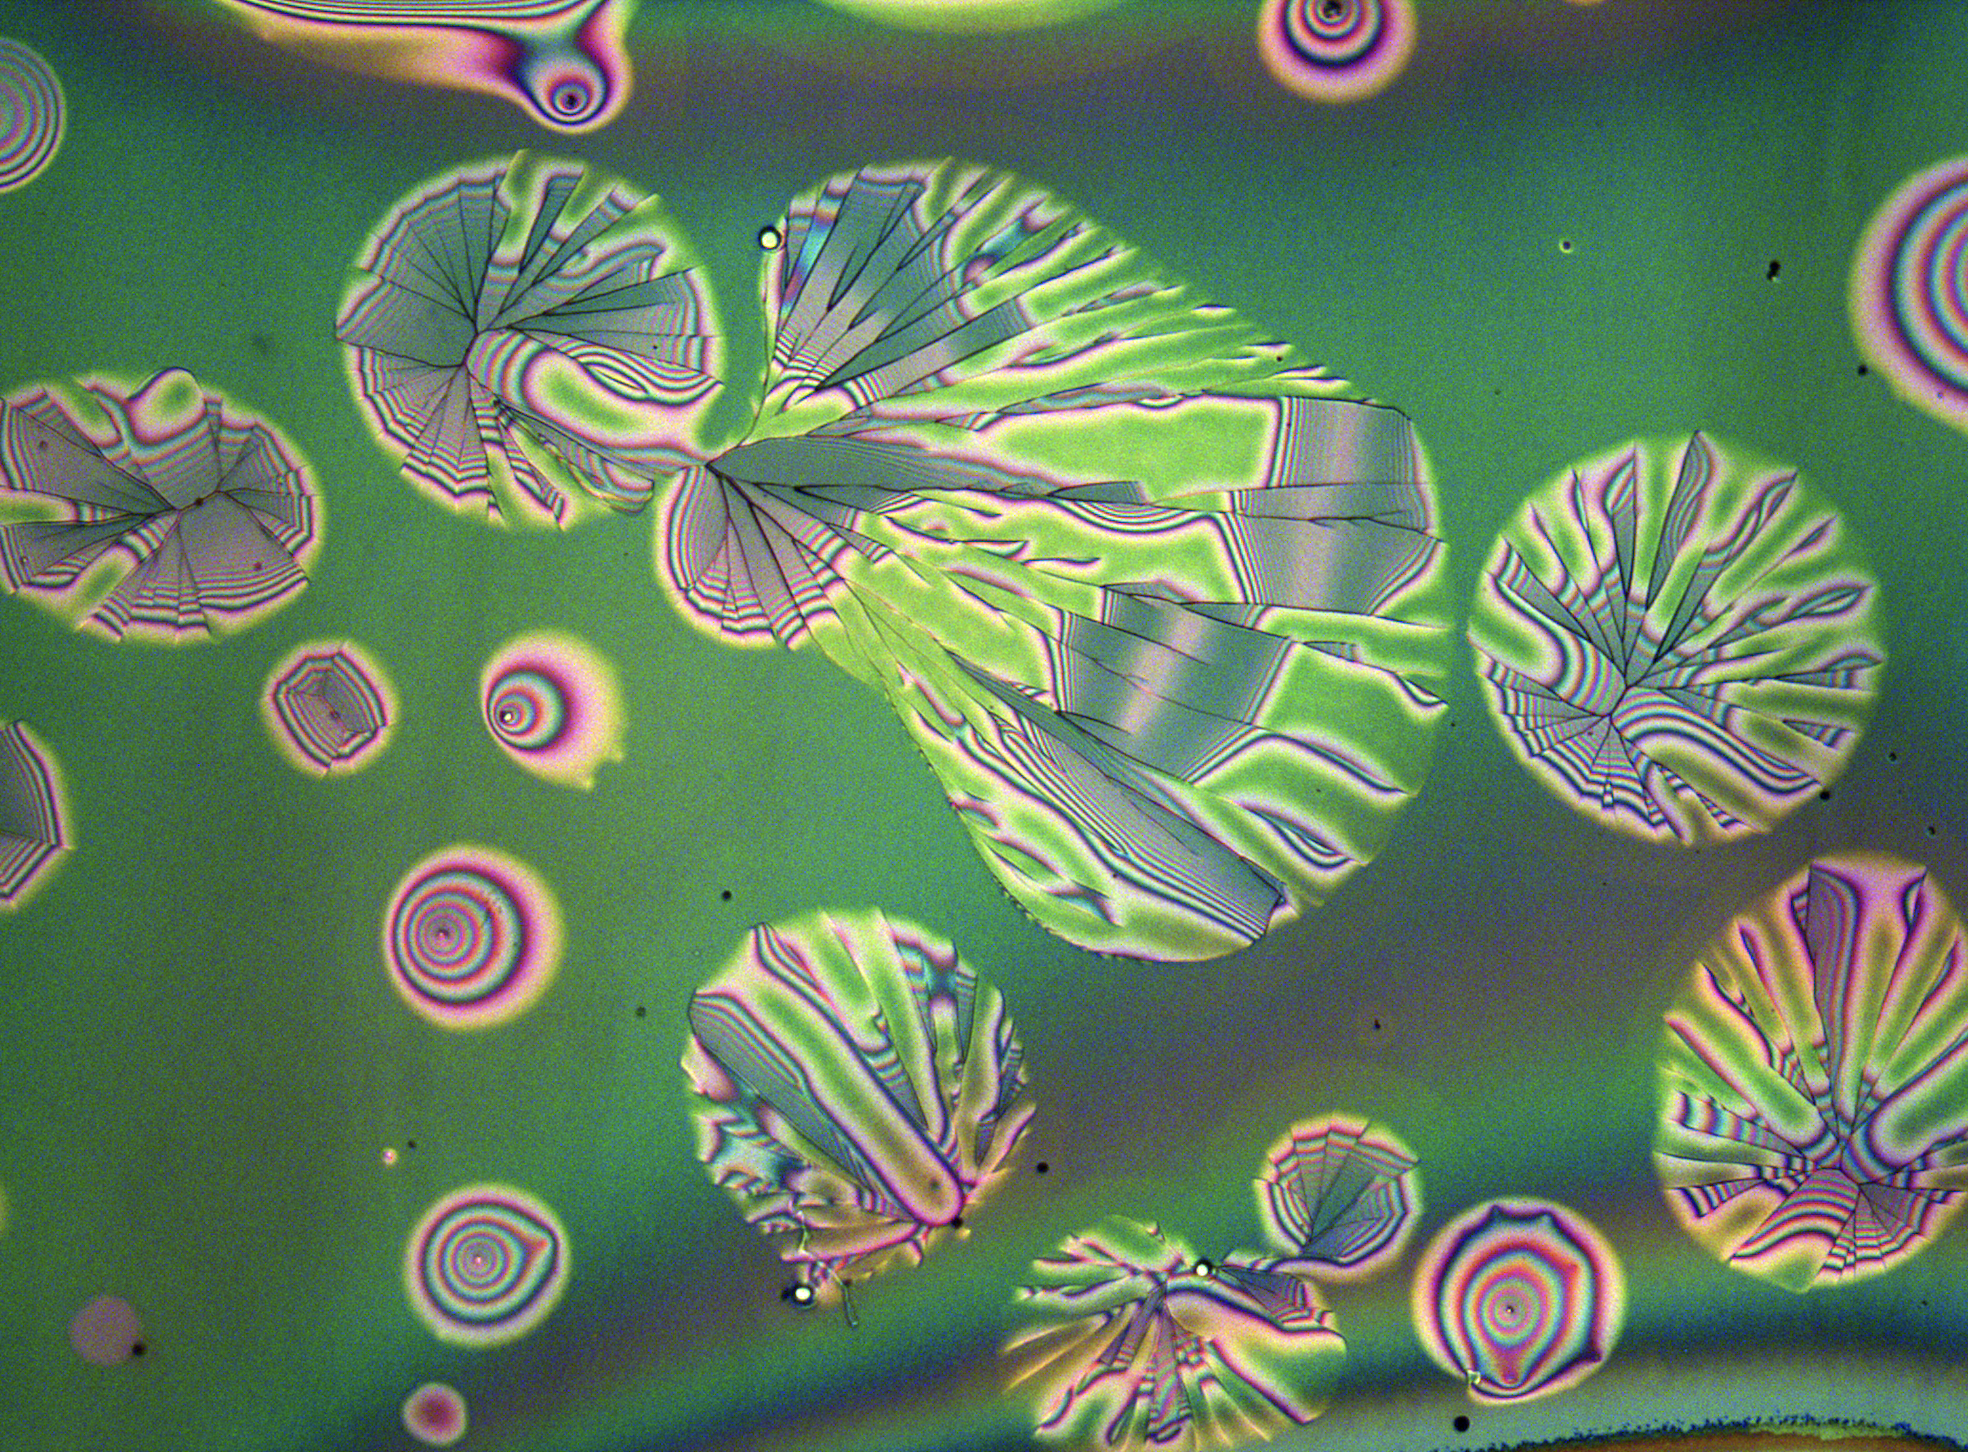
\includegraphics[width=0.45\textwidth]{figures/led_after_pecvd.png}
    \caption{Optical image of the LED.}
    \label{fig:led_optical}
\end{figure}


\subsection{Final Optical Inspection}

Using an optical microscope, the final LED sample was inspected.
\autoref{fig:best_led} shows the visually best LED, which has an 80 \textmu m period and a 4 \textmu m finger width.
\autoref{fig:worst_led} shows the visually worst LED, which has a 40 \textmu m period and a 16 \textmu m finger width.

A final 50X magnification optical image were taken of all four alignment marks.
The result can be seen in \autoref{fig:align_marks}.
From these pictures, it is not possible to give a numerical estimate on the alignment accuracy

\begin{figure}
    \centering
    \begin{subfigure}{0.49\linewidth}
        \centering
        \includegraphics[width=\textwidth]{figures/led_80_4_5x.jpg}
        \caption{Visually best LED. 80 \textmu m period and 4 \textmu m width.}
        \label{fig:best_led}
    \end{subfigure}
    \hfill
    \begin{subfigure}{0.49\linewidth}
        \centering
        \includegraphics[width=\textwidth]{figures/led_40_16_5x.jpg}
        \caption{Visually worst LED. 40 \textmu m period and 16 \textmu m width.}
        \label{fig:worst_led}
    \end{subfigure}
    \caption{5X magnification optical images of the visually best and worst LEDs.}
\end{figure}

\begin{figure}
    \centering
    \includegraphics[width=0.49\textwidth]{figures/align_marks.png}
    \caption{50X magnification optical images of the four alignment marks.}
    \label{fig:align_marks}
\end{figure}


% still in nanolab???

%%%%%%%%%%%%%%%%%%% DISCUSSION %%%%%%%%%%%%%%%%%%
\section{Discussion}
\label{discussion}
% DISCUSSION

\subsection{Photolithography}
\label{sec:discussion:photolithography}

% lithography undercut 
All the lithography processes used in this work gave valuable experience.
One of the experiences was how to do a dose test to get a sufficient undercut while using negative photoresist. 
The lab manual for the course \cite{labmanual} states that the undercut should be at least 1 \textmu m deep, while the teaching assistant stated that 0.5-1 \textmu m would be sufficient.
Getting an exact measurement of the undercut was difficult with the Table Top SEM, because the tilting and rotation of the sample in the chamber is very restricted. 
Quantification of the undercut with the Table Top SEM, but the undercut is clearly visible in the SEM image in \autoref{fig:undercut}.
Estimating the undercut was easier when using the optical microscope. 
First it was assessed whether the slope visible in the optical images in \autoref{fig:undercut_top} and \autoref{fig:undercut_bot} was an undercut or not.
Over- and under focusing on the edge indicated that the slope was an undercut, and this was confirmed in the SEM. 
The quantification of the undercut was done by measuring the length of the slope and comparing this to the width of the finger. 
This is a crude approximation, but it confirmed that the undercut was in the range of 0.5-1.5 \textmu m, assuming that the widest part of the finger was 5 \textmu m wide.


% negative vs positive resist
If all the photolithography steps were done again from start, positive photoresist would have been preferred over negative photoresist to get the best possible results.
All the steps with positive photoresist gave better results than with negative photoresist.
One example of the bad xxxxx
Negative photoresist is supposed to be better to use for lift-off, because of the undercut, but it was concluded that the positive resist gave sufficiently good results and less edge problems when used in the lift-off process.
One of the students did use positive photoresist for the lift-off process in his project thesis, and found there too that the positive resist gave good enough results.


\subsection{Etch}
\label{sec:discussion:etch}

% the etch curves which are not flat
The plots from the profilometer on the etches show that the etch is not perfectly flat.
Three artifacts have been identified in the etch process, which are the cause of the non-flat etch.

One artifact is the contact loss shown in \autoref{fig:Dummy_GaAs_80nm_etch_lost_contact}. 
Here the depth is measured to 80 nm, but this is uncertain since the contact is lost.
The contact loss can be countered with the right settings on the profilometer. 
The artifact could have been something else, but the contact loss is the most likely cause since the profilometer data outside the plot on the left side is flat and correct. 

A second artifact are on the vertical edges, where the etch is varying a lot. 
This is illustrated in \autoref{fig:profilometer_GaAs_100nm_etch}.
The other vertical edges varied in other but similar ways. 
This could both be caused by the etch process and the profilometer.
The profilometer might struggle to measure around vertical edges. 
The etch process could be affected by  the increased area and by different etch rates on different crystallographic planes.

A third artifact is the squiggly surface, shown between the fingers in \autoref{fig:profilometer_GaAs_100nm_etch}. 
This artifact is caused by the etch process, and is present all over the wafer where the etch was done. 
The surface is varying around $\pm$ 5 nm, which is a lot for a 100 nm etch.
This artifact could potentially block some of the light from the LED, but it is not clear how much of the light this could block.

\subsection{Deposition of Passivation Layer} 
If all process steps are done correctly, the LED will emit light at 675 nm.  
For Si$_3$N$_4$, this corresponds to an optical thickness of around 250 nm.
The optical thickness of Si$_3$N$_4$ was measured to be 249.70 nm and calculated to be 247.91 nm.
This is very close to the target, which is good.
It is also expected that the values are close.

In order to adjust the thickness to get even closer to the target thickness, the deposition time could be adjusted.
The deposition time was 18 minutes and 35 seconds.
This corresponds to a deposition rate of 0.22 nm/sec, assuming that the deposition was linear and that the measured thickness is correct.
Using these numbers, the deposition time could be adjusted to 18 minutes and 36 seconds, which would give an optical thickness of 249.9 nm, slightly closer to target value.

%Adding a passivation layer % https://www.sciencedirect.com/topics/engineering/passivation-layer




\subsection{Surface artifact}
\label{sec:discussion:surface_artifact}

The surface of the LED was far from perfect throughout the process.
While alignment in the MLA was done, multiple surface impurities were visible. 
These impurities are probably what is seen as a high and abrupt peak in the profilometer data in \autoref{fig:profilometer_GaAs_100nm_etch} around 320 \textmu m.
Peaks like this one are visible in all the profilometer data from the sample. 
The optical microscope images in \autoref{fig:led_optical} show that the surface have many surface impurities which have cracked before, during or after annealing. 


The annealing process made the surface artifacts and more visible.
It is most likely that the surface impurities were present before the etch, and that the etch process has made the area around the impurities more susceptible to cracking and slightly different etch rates.
The different etch rates are visible as different colors in the optical microscope images in \autoref{fig:led_optical}, which can arise due to different thicknesses. 
Another argument for the artifacts being a result of the etch process and not the annealing, is that the passivation layer totally covers the surface and protects it from damage. 






%%%%%%%%%%%%%%%%%%% CONCLUSION %%%%%%%%%%%%%%%%%%
\section{Conclusion}
\label{conclusion}
% Conclusion

% This is the abstract

% Light emitting diodes (LED) are widely used light producing electrical components.
% % The production of such devices .... smt nanotechnology?
% In this rapport, a premade multi-layered semiconductor wafer is used to produce LEDs.
% The wafer have been processed by strategically using photolithography, deposition, and etching.
% The LED have been characterized using an optical microscope, a scanning electron microscope, a profilometer, an ellipsometer and a SourceMeter.
% Measurements of the IV-characteristics of the LEDs have been performed, which confirmed that the LEDs are working as a diode, and they are emitting light.
% With voltage at 1.7 V and current at 30 mA the LEDs emits red light, which is the around the target wavelength of 675 nm.


% This is the conclusion
Functioning LEDs have been produced by using a multi-layered semiconductor wafer.
The wafer have been processed by strategically using photolithography, deposition, and etching.
Characterization of the LEDs have been performed and the results show that the LEDs are working as a diode.
With voltage at 1.7 V and current at 30 mA the LEDs emits red light, which is the around the target wavelength of 675 nm.

%%%%%%%%%%%%%% REFERENCES %%%%%%%%%%%%%%%%%%
}
\begingroup
\begin{center}
  \rule{2cm}{.4pt}
\end{center}
\makeatletter
\@beginparpenalty=10000
\makeatother
\bibliographystyle{unsrt} %unsrtnat
\bibliography{references}


\endgroup

\end{document}